\documentclass[11pt]{article}

\usepackage[utf8]{inputenc}
\usepackage[T1]{fontenc}
\usepackage[english]{babel}
\usepackage{amsmath,amssymb}
\usepackage{geometry}
\usepackage{booktabs}
\usepackage{url}
\usepackage{xspace}
\usepackage{hyperref}
\usepackage{natbib}
\usepackage{tikz}
\usetikzlibrary{positioning,arrows.meta,calc}

\hypersetup{colorlinks=true, linkcolor=blue!60!black, citecolor=blue!60!black,
  urlcolor=blue!60!black, pdfauthor={Chong Liu}}

\geometry{margin=2.4cm}

\newcommand{\pkg}{\textsc}
\newcommand{\air}{\pkg{Academic Integrity Recorder}\xspace}
\newcommand{\evpkg}{\textsc{Evidence Package~v1}\xspace}
\newcommand{\jcs}{\textsc{RFC\,8785 JCS}\xspace}
\newcommand{\aead}{\textsc{XChaCha20-Poly1305}\xspace}
\newcommand{\ed}{\textsc{Ed25519}\xspace}
\newcommand{\argon}{\textsc{Argon2id}\xspace}

\title{Unforgeable Process Evidence:\\ A New Paradigm of Scientific Integrity\\ Complementing Reproducibility}

\author{Chong Liu\thanks{Corresponding author. Independent Researcher.
ORCID: 0009-0009-8116-1255. Email: chong.liu.phil@outlook.com.
Code and specification: \url{https://github.com/chongliuresearch/academic-integrity-recorder}.}}

\date{\today}

\begin{document}

\maketitle

\begin{abstract}
Reproducibility has become the dominant frame for scientific integrity: a result is
trusted insofar as an independent party can rebuild it from shared data and code. We
argue that reproducibility verifies \emph{what} was claimed but remains silent about
\emph{how} the claim was arrived at, and that this second question is a distinct and
complementary axis of integrity that the present crisis exposes without resolving. We
propose \emph{unforgeability} as the operative property of that axis: evidence about the
research process that is computationally infeasible to fabricate or retroactively
alter, so that a validated record is itself non-trivial evidence that the reported
process occurred as and when it is attested to have occurred. We develop the scientific
rationale for treating unforgeable process evidence as a new paradigm of scientific
integrity---a support for truth-claims that complements, rather than replaces,
reproducibility---and we show that the
property is technically achievable today with local, privacy-preserving, cryptographic
recording that any third party can verify offline. We make the claim concrete through a
proof-of-concept exemplar: an open specification (\evpkg) and a prototype reference
implementation (\air), released as open source and open to community contribution.
Throughout, we are careful about what unforgeability
does \emph{not} establish: it attests process integrity, not truth, originality,
authorship, or completeness. We close with scope, limitations, and a governance path for
adoption.
\end{abstract}

\section{Introduction}
\label{sec:intro}

The reproducibility crisis is usually told as a story about \emph{results}: too many
published findings cannot be rebuilt from the materials that authors share
\citep{nosek2015top,donoho2009}. The standard remedy has therefore been to share
more---data, code, protocols, preregistrations---so that an independent party can
re-derive the outcome \citep{nosek2015top,donoho2009}. This framing has made
\emph{reproducibility} the de facto currency of scientific integrity: a result is
trustworthy to the extent that it can be regenerated.

We propose a complementary frame. Reproducibility answers the question
\textit{``can the result be rebuilt?''} It does not answer \textit{``was the result
arrived at honestly?''} A finding can be perfectly reproducible and yet be the product
of selective reporting, post-hoc hypothesizing, undisclosed reuse of a collaborator's
work, or an AI-assisted draft presented as original. Conversely, a genuinely honest
workflow may fail to reproduce for reasons unrelated to misconduct---fragile materials,
unreported environmental conditions, or legitimate stochasticity \citep{ioannidis2005}.
The two questions are correlated but distinct, and the crisis literature documents the
blind spot explicitly: even when a study is replicated, an observer cannot tell whether
the \emph{process} that produced the original was faithful \citep{john2012,fanelli2009}.

What is missing, we argue, is not another call for transparency but a precise,
checkable property. We call that property \emph{unforgeability}. A process-evidence
record is unforgeable if it is computationally infeasible---under explicitly stated
assumptions---to produce a record that validates for a process that did not actually
occur, or to alter, reorder, or backdate an existing record without detection. Under
this property, successful validation of a record becomes non-trivial evidence that the
recorded process happened as attested. Unforgeability is thus not an assertion of virtue
but a conditional, mechanistic guarantee: it narrows the set of ways a claim could be
false by removing those that depend on fabricating the process itself. It serves the
broader goal of \emph{process trustworthiness}---verifiable evidence that the conduct of
research was recorded as it happened---by giving that goal a formal, falsifiable core.

The distinction between the goal and the property matters. ``Process trustworthiness''
describes an aspiration that is easy to affirm and hard to evaluate; ``unforgeability''
names a property that a skeptic can actually check, because checking it reduces to
re-deriving hashes and signatures. A design that aims at unforgeability commits itself
to concrete mechanisms---an append-only hash chain, canonical serialization, a device
signature, and an external timestamp---each of which can fail or be attacked, and each of
which can therefore be stated and scrutinized. This is the sense in which the concept is
scientifically productive rather than merely rhetorical.

Our contributions are:
\begin{enumerate}
  \item a clear separation of \emph{reproducibility} (what was claimed) from
        \emph{unforgeable process evidence} (how the claim was arrived at), and an
        argument that the latter constitutes a new paradigm of integrity complementing
        reproducibility;
  \item a characterization of unforgeability for research-process evidence, stated as a
        conditional guarantee under explicit cryptographic and operational assumptions,
        together with its epistemic role as a complement to reproducibility;
  \item a proof-of-concept exemplar---an open \evpkg specification and a prototype
        reference implementation (\air), released as open source---demonstrating that
        the property is achievable with ordinary, local, privacy-preserving tooling;
  \item a candid treatment of scope, adversarial limits, and a governance path for
        adoption.
\end{enumerate}

\begin{quote}
\textbf{Non-claim.} Unforgeable process evidence proves process integrity---that the
recorded process occurred as recorded, on the attested device, at the attested time,
modulo the stated cryptographic assumptions. It does \emph{not} certify identity,
authorship, originality, correctness, or academic integrity, and it cannot prove that
all research activity was captured. This boundary is designed into the recording
format and its exported manifest, not merely asserted in prose.
\end{quote}

\section{The Reproducibility Crisis}
\label{sec:crisis}

\subsection{What the empirical record shows}

The crisis is not anecdotal. In a 2016 \emph{Nature} survey of 1,576 researchers,
\textbf{70\%} reported having failed to reproduce another group's experiment, and
more than half reported failing to reproduce \emph{their own} \citep{baker2016}.
Among large coordinated replications, the Open Science Collaboration reran 100
psychology studies and found only \textbf{36\%} reproduced the original statistically
significant result, with effect sizes roughly half as large \citep{osc2015}. In
preclinical cancer biology, the Reproducibility Project reproduced only a minority of
high-impact findings \citep{errington2021}, consistent with earlier industry reports
that roughly \textbf{11\%} (6 of 53) of landmark preclinical studies could be
reproduced internally \citep{begley2012} and that a major pharmaceutical pipeline
observed reproducibility in only about one fifth of projects \citep{prinz2011}.

These numbers are not a verdict on any discipline's honesty; they are a verdict on the
\emph{visibility} of process. As \citet{ioannidis2005} argued two decades ago, the
prevailing incentive structure predicts a large fraction of false positives even
without malfeasance, and \citet{john2012} documented that questionable research
practices (p-hacking, selective reporting, undisclosed flexibility) are common and
often unconscious.

\subsection{Why reproducibility alone is insufficient}

Reproducibility operates on the \emph{output} side of research. It asks whether, given
shared inputs, the same outputs reappear. Three gaps follow.

First, \textbf{the reporting gap}. Reproducibility depends on what authors choose to
share. Studies show extensive under-disclosure of experimental design, and that the
absence of a disclosure norm is itself a cause of non-reproduction
\citep{nosek2015top}. What is never written down cannot be reproduced, and the
decision of what to write down is exactly the process reproducibility cannot see.

Second, \textbf{the selectivity gap}. Even with full data, reproducibility cannot
distinguish a result obtained by pre-specified analysis from one obtained by
exploring many analyses and reporting the best \citep{ioannidis2005,gelman2014}.
Preregistration addresses this prospectively \citep{nosek2018}, but it covers a
narrow slice of ordinary research behavior and is silent about the long, messy
trail of reading, drafting, and revision that precedes any registration.

Third, \textbf{the provenance gap}. Modern research increasingly involves tools---search,
writing environments, version control, and AI assistants---whose use is rarely
disclosed in a verifiable way \citep{gao2023}. Whether and how an AI
contributed to a manuscript, whether a passage was copied from a collaborator, or
whether a figure was regenerated after peer review are questions about \emph{process},
and reproducibility is structurally blind to them.

None of this diminishes reproducibility; it motivates a second pillar that observes
the conduct of research directly rather than inferring it from its outputs.

\section{Unforgeability: Rationale and Epistemic Role}
\label{sec:rationale}

\subsection{The warrant of a scientific claim}

A scientific result functions as evidence for a claim about the world to the degree that
the process producing it can be trusted. That trust decomposes into two questions that
are easy to conflate but distinct in what they can be checked. The first asks whether
the reported result follows from the reported materials---call this the question of
\emph{reproducibility}, of \emph{what} was claimed. The second asks whether the reported
process is the \emph{actual} process---whether the experiment, the reading, the analysis,
and the writing happened as they are described, in the order described, and before the
outcome was known. Call this the question of \emph{fidelity}, of \emph{how} the claim
was arrived at. A result can score high on the first question and low on the second, and
vice versa.

Science has always treated the second question as load-bearing, even when it lacked the
machinery to answer it mechanically. The laboratory notebook is a centuries-old
technology whose entire purpose is to make the conduct of experiment visible to later
scrutiny, precisely because its contemporaneity---the fact that its entries were written
as events unfolded rather than reconstructed afterward---is what gives it evidentiary
weight \citep{macrina2014}. The W3C \textsc{PROV} model formalizes provenance as a
first-class, machine-checkable object \citep{w3cprov2013,moreau2013,moreau2013book}, and
open-science movements have long insisted that transparency of process is as important
as availability of products \citep{nosek2015top,fanelli2011}. What these strands share is
an implicit commitment to exactly the property we wish to make explicit: that the account
of how a result was produced should itself be trustworthy.

The reproducibility crisis can be read as the failure of the present ecosystem to secure
this second question. Its signature behaviors---p-hacking, HARKing, selective reporting,
the post-hoc construction of a clean narrative---do not primarily attack the
regenerability of a result; they attack the fidelity of its provenance, and they survive
reproduction precisely because a fabricated-but-consistent artifact can be re-derived
just as easily as a genuine one. Reproducibility, by construction, cannot tell the two
apart: it verifies the artifact, not the act. If the act is what matters for evidentiary
weight, then a property that binds the act---rather than the artifact---is what is missing.

\subsection{Unforgeability as the operative property}

We therefore need a property that speaks to the act rather than the artifact. We propose
\emph{unforgeability}. Informally, a process-evidence record is unforgeable if a
would-be fabricator cannot produce a record that passes validation for a process that
did not occur, nor alter an existing record---by inserting, deleting, reordering, or
backdating events---without that change being detected. The force of the definition lies
in what validation then licenses: if a record validates, then, under the assumptions on
which the property rests, the recorded process did in fact occur as recorded.

Two qualifications keep this claim honest. First, unforgeability here is
\emph{computational} and \emph{conditional}, not absolute. It rests on the hardness of
standard cryptographic primitives---collision-resistant hashing, unforgeable signatures
under the \ed scheme \citep{bernstein2012}, and authenticated encryption
\citep{bernstein2008}---and on operational assumptions such as the secrecy of signing
keys and the integrity of any external timestamp. An adversary who compromises a key, or
who controls the clock, can defeat the property, and no honest account can pretend
otherwise. Second, unforgeability is a property of the \emph{record}, not a verdict on
the \emph{research}. An unforgeable record of a flawed experiment is still a flawed
experiment. What the property does is eliminate an entire class of failures---those that
operate by fabricating or rewriting the process itself---leaving the remaining
uncertainty to methodology and interpretation, which is precisely where peer review and
replication are effective.

It is useful to contrast unforgeability with the weaker, more familiar notion of
\emph{tamper-evidence}. A tamper-evident record is one whose alteration is detectable;
that is a property of the mechanism one uses to build the record. Unforgeability is the
property of the record one wants: that no convincing counterfeit can be produced at all.
Tamper-evidence is the means; unforgeability is the end. Leading with the end clarifies
both the design goal and the security claim, and it is why we organize the exemplar in
\S\ref{sec:design} around achieving unforgeability through a hash chain, canonical
serialization, a device signature, and a timestamp---rather than merely around
detectable tampering.

\subsection{Complementarity with reproducibility}

Unforgeability is not a substitute for reproducibility; the two secure different
questions, and both are needed. The relationship is cleanest as a two-by-two space
(Table~\ref{tab:comp}). A result that is reproducible but whose process is forgeable can
be rebuilt yet may rest on a fabricated or selectively edited account. A result whose
process is unforgeably recorded but which fails to reproduce points to a problem of
method or robustness rather than of honesty---its process is attested, its inference is
doubtful. A result that is both reproducible and unforgeably recorded enjoys the
strongest available evidentiary basis short of independent corroboration of the
underlying phenomenon. And a result that is neither commands the least.

\begin{table}[ht]
\centering
\small
\begin{tabular}{@{}p{3.4cm}p{5.6cm}p{5.4cm}@{}}
\toprule
 & \textbf{Reproducible} & \textbf{Not reproducible} \\
\midrule
\textbf{Unforgeable process} &
result regenerates \emph{and} process is attested (strongest) &
process attested but result does not regenerate (method or robustness doubt) \\
\textbf{Forgeable process} &
result regenerates but process may be fabricated or edited &
neither regenerable nor attested (weakest) \\
\bottomrule
\end{tabular}
\caption{Unforgeability and reproducibility secure different questions and are
independent. Each cell indicates what the two properties jointly establish.}
\label{tab:comp}
\end{table}

Two observations follow. First, the properties are \emph{independent}: knowing that a
result reproduces tells us nothing about whether its process was genuine, and knowing
that its process was unforgeably recorded tells us nothing about whether the result will
reproduce. This independence is exactly why unforgeability contributes evidence that
reproducibility cannot supply. Second, the value of unforgeability is asymmetric and
incremental: it does not raise the ceiling of what science can claim, but it raises the
floor below which evidence cannot easily fall. By making the fabrication of process
computationally infeasible and its detection mechanical, it converts a category of
integrity failures from matters of contested testimony into matters of checkable fact.
That is a modest but genuine strengthening of the evidentiary basis on which scientific
truth-claims rest---modest, because it never establishes truth; genuine, because it
narrows the ways a claim could be false.

\subsection{Technical feasibility}

The property would be idle if it were not attainable with ordinary tooling, on ordinary
machines, without imposing surveillance. Three developments make unforgeable process
evidence practical now where it was not a decade ago.

\textbf{Local-first capture without a panopticon.} The evidence can be collected on the
researcher's own machine, with no server, no telemetry, and sensitive content never
leaving the device in cleartext. This addresses the principal objection to process
recording---that it is surveillance---and aligns with data-minimization norms
\citep{voigt2017}. Local-first is a design choice in service of unforgeability's
adoption, not a headline property: it removes the single largest reason a researcher
would refuse the tool, and thereby widens the conditions under which an unforgeable
record can exist at all.

\textbf{Cheap, standard cryptography.} Every primitive the property needs is
library-grade. An append-only hash chain commits each event to its predecessor, so
deletion, reordering, or editing breaks the chain \citep{crosby2009}. Canonical
serialization (\jcs) makes hashing independent of key order and whitespace
\citep{rfc8785}. A device signature under \ed attests the recorder and gives the record
its unforgeable anchor \citep{bernstein2012}. Authenticated encryption (\aead) seals
sensitive content \citep{bernstein2008}. An internet-independent timestamp, such as
OpenTimestamps, can later prove existence at or before a point in time without trusting
a notary \citep{opents}. None of this is exotic; all of it is battle-tested.

\textbf{Offline, adversarial verification.} Because the property is mathematical, a
skeptic needs no special access to check it. The verifier is a small, auditable program
that re-derives every hash and signature; its success, rather than any party's
assertion, is what licenses the inference that the record is genuine. This is the same
principle that makes signed commits and checksums trustworthy without a trusted third
party, and it is what distinguishes unforgeable process evidence from a self-reported
methods section, which remains forgeable however detailed it is.

\section{A Feasibility Exemplar: a Prototype Reference Implementation}
\label{sec:design}

We now illustrate---not exhaust---the argument with a deliberately brief account of
\air, an open-source \emph{prototype} of the \evpkg, released under the AGPL-3.0
license and open to community contribution. It is a proof-of-concept, not a finished
system: the specification is the stable artifact, while the code is an evolving
demonstration that the property is attainable, with deliberately partial platform
support. We therefore describe only the mechanisms that carry the argument---
\emph{unforgeability}, \emph{local-first capture}, \emph{honest capability disclosure},
\emph{privacy-by-default}, and \emph{offline verification}---and leave implementation
detail to the project itself.

\subsection{Architecture}

\begin{figure}[ht]
\centering
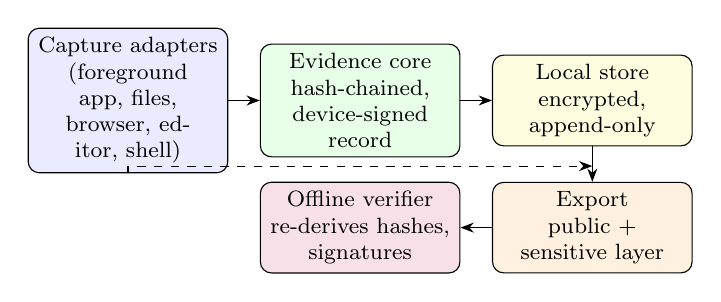
\begin{tikzpicture}[>=Stealth, node distance=0.45cm and 0.4cm,
  every node/.style={font=\footnotesize, align=center, text width=2.3cm}]
  \node[draw, rounded corners, fill=blue!8] (cap)
    {Capture adapters\\(foreground app, files,\\browser, editor, shell)};
  \node[draw, rounded corners, fill=green!9, right=of cap] (core)
    {Evidence core\\hash-chained,\\device-signed record};
  \node[draw, rounded corners, fill=yellow!12, right=of core] (store)
    {Local store\\encrypted,\\append-only};
  \node[draw, rounded corners, fill=orange!12, below=of store] (exp)
    {Export\\public + sensitive layer};
  \node[draw, rounded corners, fill=purple!12, left=of exp] (ver)
    {Offline verifier\\re-derives hashes,\\signatures};
  \draw[->] (cap) -- (core);
  \draw[->] (core) -- (store);
  \draw[->] (store) -- (exp);
  \draw[->] (exp) -- (ver);
  \draw[->, dashed] (cap.south) |- ($(exp.north)+(0,0.2)$);
\end{tikzpicture}
\caption{Sketch of the architecture. Evidence flows from capture adapters into an
evidence core that maintains a hash-chained, device-signed record, is persisted in an
append-only local store, exported as a two-layer \evpkg, and verified entirely offline.
No telemetry leaves the device.}
\label{fig:arch}
\end{figure}

Capture adapters observe activity---foreground application, file events, browser and
editor interactions, and (opt-in) shell commands. They forward events to the evidence
core, which canonicalizes, hashes, signs, and persists them (Figure~\ref{fig:arch}).

\subsection{The hash chain}

The core mechanism is an append-only hash chain. Each recorded moment is an
\emph{evidence event} carrying a sequence number, timestamps, a source, a semantic
kind, and a sensitivity label; its payload hash and the hash of the preceding event are
committed into the event's own hash. Because every link binds its predecessor, editing,
deleting, or reordering any event changes its hash and so breaks every subsequent link
and the signed head of the chain \citep{crosby2009}. The primitives are standard and
battle-tested: collision-resistant hashing, a device signature, authenticated
encryption for sensitive content, and an optional internet-independent timestamp to
prove existence at or before a point in time
\citep{rfc8785,bernstein2012,bernstein2008,opents}. Events are persisted as immutable,
append-only encrypted segments with signed checkpoints of the chain head; a crash is
reconciled on open, and unsigned, missing, or reordered segments are rejected, so
history cannot be silently rewritten.

\subsection{Export and honest disclosure}

Export produces a single \evpkg with a signed manifest and two layers. The \emph{public
layer} carries the event chain with payloads replaced by their hashes and a
human-readable report, so integrity can be checked without revealing content; the
\emph{sensitive layer} holds the full events, artifacts, and disclosures, sealed under
a passphrase-derived key. The manifest states exactly what the package claims---and,
just as important, what it does not.

The design's distinctive mechanism is \emph{honest capability disclosure}. Each capture
capability is reported as \textsc{Available}, \textsc{PermissionRequired},
\textsc{Degraded}, or \textsc{Unavailable}, and any lapse in coverage is recorded as an
explicit \texttt{Gap} event rather than silently omitted \citep{air2026}. A research
claim can also be \emph{anchored} to a specific passage of a manuscript and later
revalidated, and an \emph{active-time} measure reports a conservative lower bound on
observed foreground activity. This honesty is what makes the record trustworthy: it is
explicit about where it stops.

\subsection{Offline verification}

Because the property is mathematical, a skeptic can check it without special access: a
small, auditable verifier re-derives every hash and signature from the package alone,
and its success---not any party's assertion---licenses the inference that the record is
genuine. Success proves \emph{process integrity and a device signature only}, and the
verifier's own output says so.

\section{Scope, Limitations, Governance, and Adoption}
\label{sec:scope}

\subsection{Scope and what the record can show}

Unforgeable process evidence is most valuable where the contested question is \emph{how},
not \emph{whether}: disclosure of AI assistance, provenance of a passage, the trail of
revision, the existence of a planned experiment that was later dropped, or a
contemporaneous lab record. It strengthens theses, grant reports, and post-publication
audit alike.

\subsection{Limits of the property}

Unforgeability is powerful but bounded, and the bounds belong to the property itself,
not to any particular implementation.

\begin{itemize}
  \item \textbf{Computational and conditional.} The property holds only while signing
        keys remain secret and any external timestamp is honest; a compromised key or a
        controlled clock can retrospectively undermine the record. Unforgeability is a
        guarantee under assumptions, not an absolute.
  \item \textbf{Attests process, not truth.} An unforgeable record shows that the
        recorded process occurred as recorded. It does not establish that the result is
        true, the method correct, or the work original; a faithfully recorded but flawed
        experiment remains flawed.
  \item \textbf{No completeness.} The property secures what was \emph{recorded}, not
        that \emph{everything} was recorded. Activity outside the instrumented
        environment is invisible to it, and no design can convert an absence of evidence
        into evidence of absence.
  \item \textbf{Not identity or authorship.} A device signature attests a key, not a
        legal person; it cannot distinguish the key's owner from anyone else using the
        device or account.
  \item \textbf{Cannot close the environment.} A determined adversary may work on
        uninstrumented machines or fabricate inputs before they are recorded; the
        property narrows the ways a claim can be false but does not eliminate every one.
  \item \textbf{Complements, not substitutes, review.} The record is evidence to be
        weighed alongside reproducibility and peer review, never a verdict on merit.
\end{itemize}

These limits are features when stated plainly: unforgeable evidence is trustworthy
\emph{because} it is explicit about where it stops.

\subsection{Governance and adoption path}

We propose unforgeable process evidence as a lightweight, open community standard, in
the spirit of how code signing and transparency logs became default expectations
\citep{crosby2009}. Concrete steps:

\begin{enumerate}
  \item \textbf{Open specification and interop.} The format and its verification are
        specified openly, so any archive or journal can check a deposited package
        without vendor lock-in \citep{air2026}.
  \item \textbf{Complement, don't replace.} Tie the record to existing norms: the
        data-availability statement, the preregistration, and the conflicts/disclosure
        form. The AI-disclosure entity maps directly onto emerging AI-use policies
        \citep{gao2023,cope2023}.
  \item \textbf{Tiered adoption.} Start with self-archiving and reviewer-on-request,
        then optional journal encouragement, then (where appropriate) a deposition
        requirement for certain claim types. Voluntary, low-friction adoption avoids the
        surveillance objection.
  \item \textbf{Incentives for honesty.} Because gaps are recorded, a complete,
        gap-light record becomes a positive signal; a record full of disclosed gaps is
        at least honest, which is more than the current default of silence.
\end{enumerate}

\section{Conclusion}
\label{sec:conclusion}

Reproducibility verifies \emph{what} was claimed; unforgeable process evidence verifies
\emph{how} the claim was arrived at. We have argued that the second is a new paradigm of
scientific integrity---not a replacement for reproducibility but a partner to it, closing
the gap that reproducibility, by construction, cannot see.
The property is attainable today with local, privacy-preserving, cryptographic recording
and offline adversarial verification, as an open specification and a prototype
implementation demonstrate, and it is honest about where it stops: it attests process
integrity, never truth, originality, or authorship. Adopting unforgeable process evidence
will not end the reproducibility
crisis, but it gives the scientific community a new instrument for the part of integrity
that reproducibility was never designed to observe.

\section*{Acknowledgments}
\label{sec:ack}
The author thanks the open-source and open-science communities whose tools and norms
this work builds upon. The prototype reference implementation is released under the
AGPL-3.0 license and welcomes community contribution.

\bibliographystyle{plainnat}
\bibliography{refs}

\end{document}
